% =============================================================================
% Updated manuscript sections -- NICEDT-2027
% "Federated Learning for Aircraft Engine Prognostics: An Analysis of Accuracy,
%  Communication, and Data Heterogeneity Trade-offs"
%
% Drop-in LaTeX (Springer LNCS compatible). Requires \usepackage{graphicx}.
% Every number comes from results/v2/paper_tables/ (5 seeds, mean +/- SD) and was
% checked automatically against results/v2/tables/summary.csv
% (python paper/check_numbers.py). Figures: paper/figures/*.pdf.
% Primary policy everywhere: validation-selected checkpoint.
% =============================================================================

% -----------------------------------------------------------------------------
\begin{abstract}
Airlines hold fleet sensor data they may be unwilling to pool, which motivates
federated learning (FL) for remaining-useful-life (RUL) prediction. We study
Federated Averaging (FedAvg) with a two-layer LSTM on NASA C-MAPSS FD001 under a
controlled protocol: every method receives the same model, preprocessing,
validation engines, training budget and checkpoint-selection rule, and every
configuration is repeated with five matched random seeds. FedAvg with five clients
reached a test RMSE of $13.24 \pm 0.32$ cycles, against $14.46 \pm 0.44$ for
pooled centralized training and $16.28 \pm 0.50$ for an operator training only
on its own 18 engines. An ablation indicates that FedAvg's advantage over
centralized training reflects the regularising effect of model averaging under
untuned shared hyper-parameters, not an intrinsic benefit of decentralisation.
The clearest benefit of federation is over local-only training, which it
improves in every seed. Accuracy improved with communication rounds up to $R=20$
and did not improve monotonically with the number of clients. Strong label and
quantity skew ($\alpha=0.1$) and whole-engine ownership each cost about
0.6--0.8~cycles of RMSE. The model update is 864{,}260~bytes, so the
primary configuration exchanges an estimated 172.85~MB.
\keywords{Federated learning \and Remaining useful life \and C-MAPSS \and
Prognostics \and LSTM \and Data heterogeneity}
\end{abstract}

% -----------------------------------------------------------------------------
\section{Experimental Protocol}\label{sec:protocol}

\paragraph{Data and preprocessing.}
We use the FD001 subset of NASA C-MAPSS (100 training and 100 official test
engines; one operating condition, one fault mode). Inputs are the three
operational settings and 14 sensors (sensors 1, 5, 6, 10, 16, 18 and 19 removed
a priori), i.e.\ 17 features. The target is the piece-wise linear RUL capped at
125 cycles. Ten of the 100 training engines are held out for validation at the
engine level (fixed split, identical for all methods and seeds), leaving 90
training engines and 15{,}630 sliding windows of 30 cycles (stride 1). A
min--max scaler is fitted on the 90 training engines only. Each test engine is
represented by its last 30 cycles, and its ground-truth RUL (capped at 125) is
used only after model selection.

\paragraph{Model and training.}
All methods use the same LSTM (two layers, 128 hidden units, dropout 0.2,
fully connected head $128\to64\to1$; 215{,}681 parameters), Adam (learning rate
$10^{-3}$, weight decay $10^{-5}$), batch size 256, gradient-norm clipping at 1,
MSE loss and a constant learning rate. No hyper-parameter was tuned for any method.

\paragraph{Methods and matched budget.}
(i) \emph{Centralized}: one model trained on all pooled training windows.
(ii) \emph{FedAvg}: $K$ clients, $R$ rounds, $E$ local epochs per round, full
participation, sample-size-weighted averaging; each client re-initialises its
Adam state every round because optimiser state is not communicated.
(iii) \emph{Local-only}: each client trains alone on its own shard; we report the
mean over the $K$ client models. Every method makes the same $R\times E=100$
passes over its training data (centralized: 100 epochs). All methods are
validated on the same ten held-out engines every $E$ epochs (i.e.\ after every
FedAvg round). The checkpoint with the lowest validation RMSE is evaluated once
on the test set. The original protocol (centralized with early stopping, FL with
a fixed budget) confounded these comparisons and is reported only as a reference.

\paragraph{Client partitions.}
\emph{IID window}: all training windows are randomly split into $K$ equal shards.
Overlapping windows of the same engine fall on different clients, so every
client sees fragments of all 90 engines.
\emph{Dirichlet window}: RUL labels are binned into ten equal-width bins, and
per-bin client shares are drawn from $\mathrm{Dir}(\alpha\mathbf{1}_K)$ with
$\alpha\in\{1.0,0.5,0.1\}$. This skews both the label distribution and the
client sizes.
\emph{Whole-engine}: the 90 training engines are randomly assigned to $K$
clients (18 each for $K=5$), so each client owns complete run-to-failure
trajectories. Every window is assigned to exactly one client and total training
data are constant across $K$. A partition is redrawn if any client receives fewer
than 256 windows (one redraw was needed for two seeds at $\alpha=0.1$).

\paragraph{Seeds and statistics.}
Each configuration is run with the same five seeds (42, 123, 2026, 3407, 9001).
A seed fixes model initialisation, the partition, mini-batch order and dropout
through independent derived streams. Runs are deterministic: repeating a seed
reproduces predictions exactly. We report mean $\pm$ sample standard deviation
over seeds, and per-seed consistency for paired comparisons. With five seeds an
exact paired test cannot reach $p<0.05$ (minimum two-sided $p=0.0625$), so we
make no claims of statistical significance.

\paragraph{Metrics.}
RMSE and MAE in cycles, and the NASA scoring function
$S=\sum_i s_i$ with $s_i=e^{-d_i/13}-1$ for $d_i<0$ and $e^{d_i/10}-1$ for
$d_i\ge0$, where $d_i=\widehat{\mathrm{RUL}}_i-\mathrm{RUL}_i$, summed over the 100
test engines.

\paragraph{Communication accounting.}
One model transfer is the serialised fp32 payload in the format used by the
Flower framework, measured as 864{,}260~bytes (862{,}724~bytes of weights plus
array headers). Each round, the server sends the model to each of the $K$ clients
and receives $K$ updates, so total traffic is $2KR\times864{,}260$~bytes. This
is an application-payload estimate. Clients were simulated in one process, so no
network traffic or protocol overhead (gRPC, TLS, TCP/IP) was measured.

% -----------------------------------------------------------------------------
\section{Results}\label{sec:results}

\subsection{Centralized, federated and local-only training}

\begin{table}[t]
\centering
\caption{Test performance on FD001 (5 seeds, mean $\pm$ SD; validation-selected
checkpoint; identical budget of 100 passes). Traffic: serialised-payload estimate.
Local-only: mean over the five client models.}\label{tab:main}
\begin{tabular}{lcccr}
\hline
Method & RMSE & MAE & NASA score & Traffic (MB)\\
\hline
Centralized (pooled data)            & $14.46\pm0.44$ & $10.67\pm0.43$ & $447.9\pm35.4$ & 0.0\\
FedAvg, IID window ($K=5$)           & $\mathbf{13.24\pm0.32}$ & $\mathbf{9.78\pm0.21}$ & $\mathbf{304.0\pm26.6}$ & 172.9\\
Local-only, IID window               & $14.58\pm0.17$ & $10.81\pm0.09$ & $414.6\pm20.4$ & 0.0\\
FedAvg, whole-engine ($K=5$)         & $13.87\pm0.19$ & $10.15\pm0.13$ & $349.0\pm26.5$ & 172.9\\
Local-only, whole-engine             & $16.28\pm0.50$ & $12.13\pm0.26$ & $651.8\pm80.3$ & 0.0\\
\hline
\multicolumn{5}{l}{\emph{Reference and ablation}}\\
Centralized, original early stopping & $14.55\pm0.48$ & $10.87\pm0.24$ & $441.4\pm61.3$ & 0.0\\
FedAvg $K=1$ (optimizer reset only)  & $13.94\pm0.89$ & $10.35\pm0.66$ & $388.1\pm99.6$ & 34.6\\
\hline
\end{tabular}
\end{table}

\begin{figure}[t]
\centering
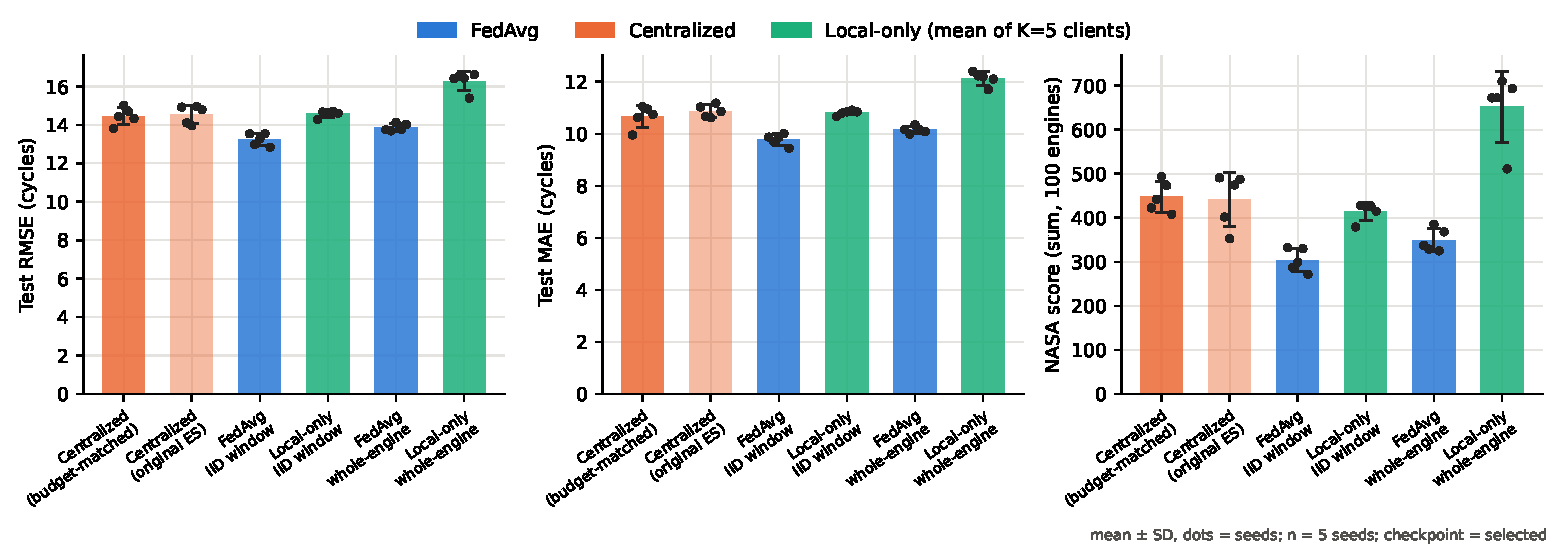
\includegraphics[width=\textwidth]{figures/fig1_main_comparison_selected.pdf}
\caption{Test RMSE, MAE and NASA score per method (bars: mean $\pm$ SD over five
seeds; dots: individual seeds).}\label{fig:main}
\end{figure}

\paragraph{Federation versus local-only training.}
Federation helps most compared with training in isolation
(Table~\ref{tab:main}). Under whole-engine ownership, an operator training only on
its own 18 engines reaches an RMSE of $16.28\pm0.50$ and a NASA score of
$651.8\pm80.3$. FedAvg on the same partition reaches $13.87\pm0.19$ and
$349.0\pm26.5$, lower in all five seeds. Local models in the IID-window split
($14.58\pm0.17$) are also worse than FedAvg in every seed. That split is less
realistic, however, because each shard contains fragments of every engine.

\paragraph{Federated versus centralized training.}
FedAvg-IID had a lower test RMSE than centralized training in all five matched
seeds ($13.24\pm0.32$ vs.\ $14.46\pm0.44$; per-seed differences 0.29--1.73
cycles, mean 1.22). The ordering is the same at the final checkpoint
($12.88\pm0.30$ vs.\ $14.82\pm1.10$). Federation adds no information, so this
reflects the optimisation procedure. The centralized model reaches its best
validation error around epoch 45 and then overfits (Fig.~\ref{fig:conv}), while
FedAvg improves slowly until round 20. A one-client FedAvg ablation, which is
centralized training with the per-round optimizer reset, reaches
$13.94\pm0.89$. It beats FedAvg-IID in only two of five seeds and overfits after
about round 7. The reset alone therefore does not reproduce the effect. The
results are consistent with averaging several clients' updates acting as a
regulariser, each client taking about 65 instead of about 310 optimizer steps per
round. We therefore do not claim that FL is intrinsically more accurate than
centralized learning: a centralized model with tuned regularisation or training
length may close the gap. The original early-stopping protocol gives practically
the same centralized result ($14.55\pm0.48$).

\begin{figure}[t]
\centering
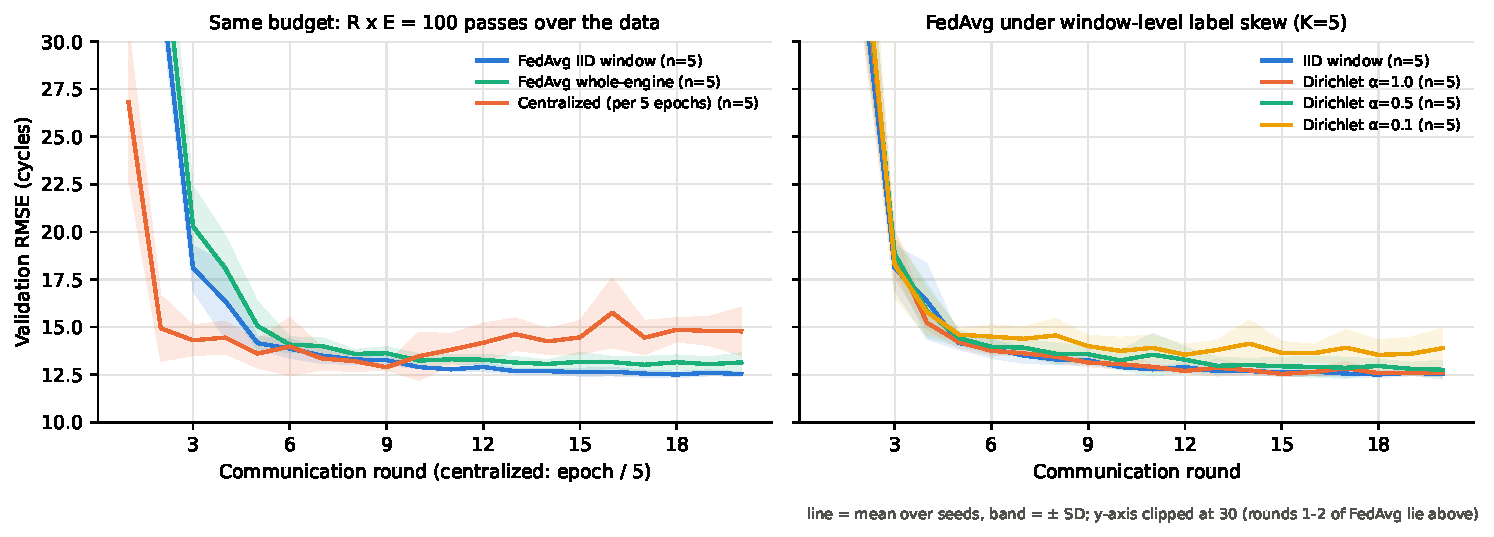
\includegraphics[width=\textwidth]{figures/fig2_convergence.pdf}
\caption{Validation RMSE per round (mean $\pm$ SD over five seeds). Left: equal
training budget; centralized plotted every five epochs. Right: FedAvg under
Dirichlet label skew.}\label{fig:conv}
\end{figure}

\subsection{Data heterogeneity and partition strategy}

\begin{table}[t]
\centering
\caption{FedAvg ($K=5$, $R=20$, $E=5$) under different partitions (5 seeds).
Client data: window counts and mean RUL across clients (range over clients and
seeds).}\label{tab:part}
\begin{tabular}{lcccc}
\hline
Partition & RMSE & NASA score & Windows/client & Client mean RUL\\
\hline
IID window        & $13.24\pm0.32$ & $304.0\pm26.6$ & 3126       & 78.1--81.8\\
Dirichlet $\alpha=1.0$ & $13.35\pm0.26$ & $309.0\pm8.7$  & 1521--5855 & 45.6--102.2\\
Dirichlet $\alpha=0.5$ & $13.47\pm0.32$ & $319.6\pm32.1$ & 1433--7250 & 42.3--105.7\\
Dirichlet $\alpha=0.1$ & $14.06\pm0.46$ & $346.4\pm34.9$ & 479--8555  & 20.8--112.8\\
Whole-engine      & $13.87\pm0.19$ & $349.0\pm26.5$ & 2751--3352 & 73.5--82.8\\
\hline
\end{tabular}
\end{table}

Moderate label skew had little effect: $\alpha=1.0$ and $\alpha=0.5$ are within
about one standard deviation of IID (Table~\ref{tab:part}). At $\alpha=0.1$ the
RMSE rose by 0.82 cycles. That partition is, however, skewed in both label
distribution (client mean RUL 20.8--112.8 cycles) and size (479--8{,}555 windows),
so the loss cannot be attributed to label heterogeneity alone. Whole-engine
ownership cost $0.63\pm0.42$ cycles relative to the IID-window split, consistently
across seeds. This gap is \emph{not} due to label heterogeneity, because client RUL
distributions are nearly identical (Fig.~\ref{fig:clients}). It reflects
differences that the window-level split introduces: every IID client sees
fragments of all 90 engines, and overlapping windows of an engine are spread
across clients. Window-level splits therefore overestimate what operators that own
whole engines can achieve, and the whole-engine setting is the more realistic one.

\begin{figure}[t]
\centering
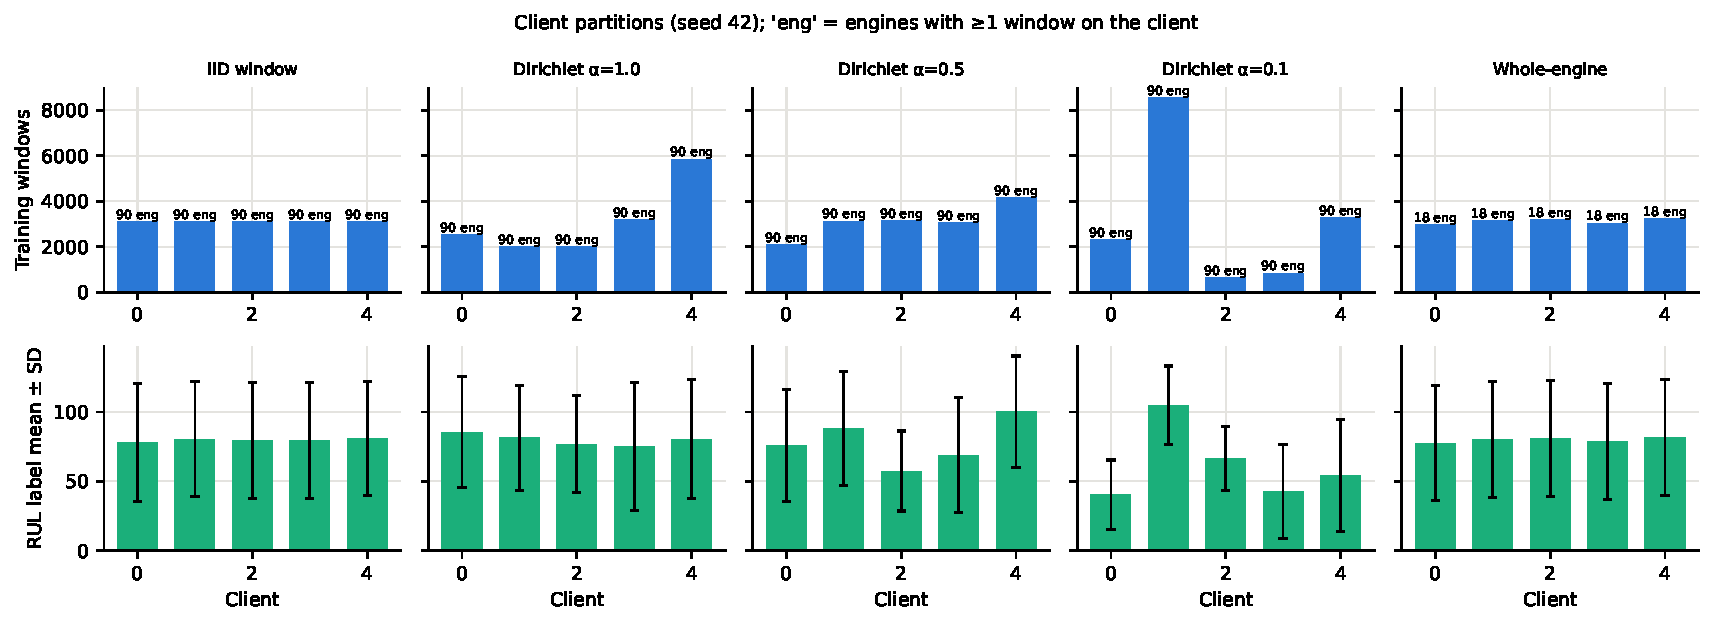
\includegraphics[width=\textwidth]{figures/fig9_client_partitions.pdf}
\caption{Client training windows (top; labels: engines with at least one window
on the client) and RUL label mean $\pm$ SD (bottom) for each partition (seed 42).}\label{fig:clients}
\end{figure}

\subsection{Communication rounds, local epochs and number of clients}

\begin{table}[t]
\centering
\caption{Parameter sweeps (FedAvg, 5 seeds, validation-selected checkpoint). One
setting varies per block; the others are fixed at $K=5$, $R=20$, $E=5$, IID
window. Total training data are fixed when $K$ varies.}\label{tab:sweeps}
\begin{tabular}{llcccr}
\hline
Sweep & Setting & RMSE & MAE & NASA score & Traffic (MB)\\
\hline
Rounds       & $R=5$  & $14.83\pm0.94$ & $11.33\pm0.75$ & $415.7\pm92.8$ & 43.2\\
             & $R=10$ & $13.78\pm0.26$ & $10.03\pm0.23$ & $338.8\pm19.1$ & 86.4\\
             & $R=20$ & $13.24\pm0.32$ & $9.78\pm0.21$  & $304.0\pm26.6$ & 172.9\\
             & $R=30$ & $13.48\pm0.31$ & $10.01\pm0.19$ & $331.1\pm29.8$ & 259.3\\
\hline
Local epochs & $E=1$  & $17.58\pm1.30$ & $13.08\pm0.83$ & $713.9\pm241.5$ & 172.9\\
             & $E=3$  & $13.44\pm0.30$ & $9.95\pm0.10$  & $307.7\pm28.3$ & 172.9\\
             & $E=5$  & $13.24\pm0.32$ & $9.78\pm0.21$  & $304.0\pm26.6$ & 172.9\\
             & $E=10$ & $13.56\pm0.37$ & $10.21\pm0.28$ & $326.6\pm30.4$ & 172.9\\
\hline
Clients, IID window & $K=2$  & $14.14\pm0.62$ & $10.47\pm0.43$ & $384.2\pm77.1$ & 69.1\\
             & $K=5$  & $13.24\pm0.32$ & $9.78\pm0.21$  & $304.0\pm26.6$ & 172.9\\
             & $K=10$ & $13.53\pm0.32$ & $9.91\pm0.08$  & $317.1\pm30.4$ & 345.7\\
\hline
Clients, whole-engine & $K=2$  & $13.65\pm0.41$ & $10.29\pm0.43$ & $327.6\pm38.3$ & 69.1\\
             & $K=5$  & $13.87\pm0.19$ & $10.15\pm0.13$ & $349.0\pm26.5$ & 172.9\\
             & $K=10$ & $14.34\pm0.59$ & $10.63\pm0.55$ & $374.7\pm62.6$ & 345.7\\
\hline
\end{tabular}
\end{table}

\paragraph{Rounds.}
RMSE fell from $14.83\pm0.94$ ($R=5$) to $13.24\pm0.32$ ($R=20$) and did not
improve further at $R=30$ ($13.48\pm0.31$), which costs 50\% more traffic
(Table~\ref{tab:sweeps}, Fig.~\ref{fig:rounds}). Because $E$ is fixed, more rounds
also means more training, so this sweep combines communication frequency with
training length. $R=10$ is within about 0.5 cycles of the best setting at half
the traffic.

\paragraph{Local epochs.}
One local epoch per round is clearly insufficient ($17.58\pm1.30$). $E=3$, $5$ and
$10$ give similar errors ($13.44$, $13.24$, $13.56$), with $E=5$ lowest on average.
Adding local computation at a fixed communication budget therefore helps only up
to a point.

\paragraph{Number of clients.}
With total data held fixed, accuracy did not improve monotonically with the
number of clients. In the IID-window split $K=5$ was best ($13.24\pm0.32$), with
$K=2$ ($14.14\pm0.62$) and $K=10$ ($13.53\pm0.32$) worse. Under whole-engine
ownership the error rose steadily as the 90 engines were divided among more
owners: $13.65\pm0.41$, $13.87\pm0.19$ and $14.34\pm0.59$ for 45, 18 and 9
engines per client. Traffic grows linearly with $K$.

The validation-selected and final-round checkpoints lead to the same conclusions
for every sweep. For example, the final-round RMSE is $12.88\pm0.30$ at $R=20$
vs.\ $13.33\pm0.22$ at $R=30$.

\begin{figure}[t]
\centering
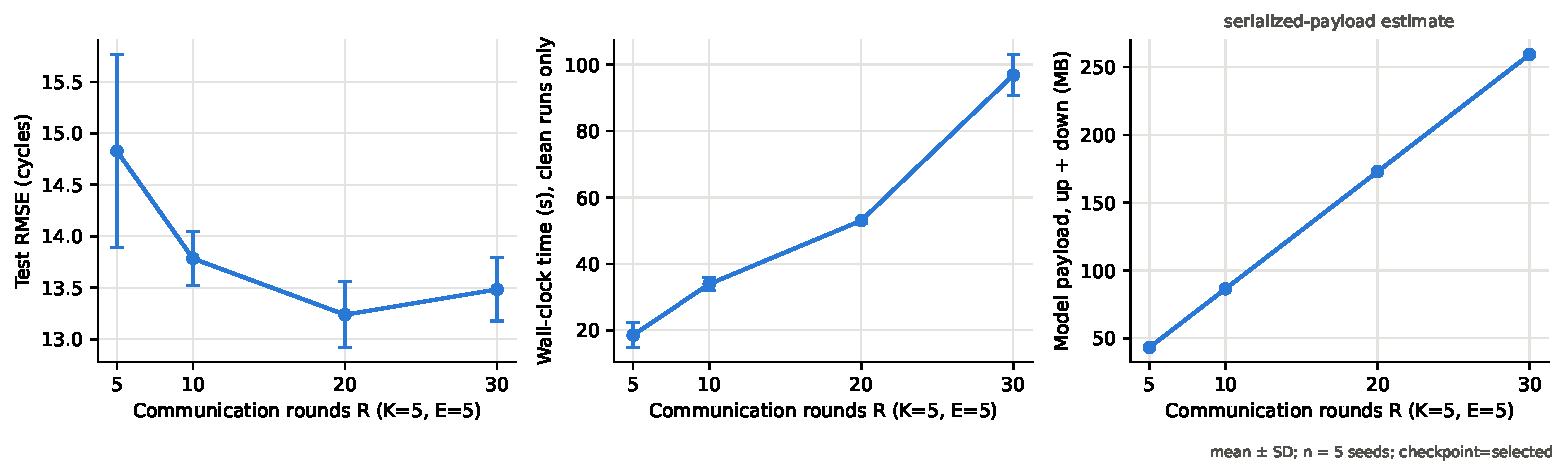
\includegraphics[width=\textwidth]{figures/fig4_sweep_rounds_selected.pdf}
\caption{Effect of communication rounds on test RMSE, wall-clock time and model
traffic (mean $\pm$ SD over five seeds).}\label{fig:rounds}
\end{figure}

\begin{figure}[t]
\centering
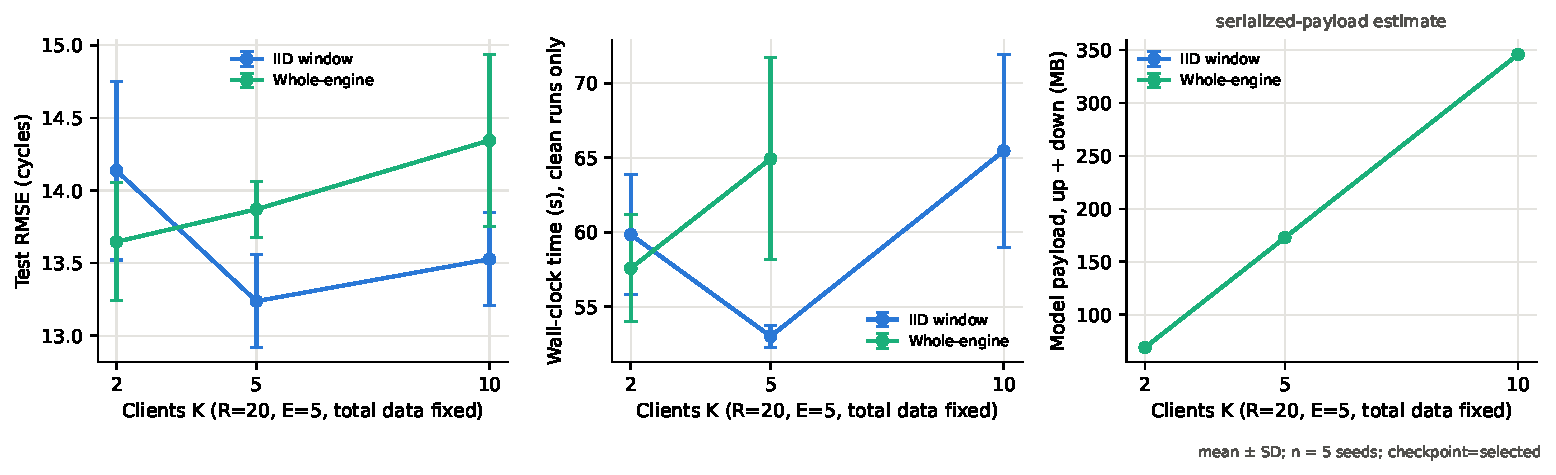
\includegraphics[width=\textwidth]{figures/fig6_sweep_clients_selected.pdf}
\caption{Effect of the number of clients with total training data fixed:
IID-window versus whole-engine partitions.}\label{fig:clients_sweep}
\end{figure}

\subsection{Communication and computation}

The primary configuration ($K=5$, $R=20$) exchanges an estimated 86.43~MB upstream
and 86.43~MB downstream (172.85~MB in total). Centralising the raw training data
would instead require about 1.3~MB as float32, roughly 130 times less. On FD001,
FedAvg is therefore motivated by data ownership, not by bandwidth savings. With
the same 100 passes over the data, centralized and FedAvg training required the same
compute (78~s and 72~s of sequential GPU time, NVIDIA RTX~4060 Laptop). If clients
ran in parallel, FedAvg would take an estimated 15.8~s (about 0.7~s per client per
round, excluding network latency).

% -----------------------------------------------------------------------------
\section{Discussion and Limitations}\label{sec:limitations}

Under matched conditions, federation is clearly beneficial compared with
operators training alone, and it is competitive with pooled training. The size of
the latter gap depends on how well the centralized baseline is regularised. All
methods over-predict RUL on average (mean error +3.3 to +4.8 cycles), which
drives the NASA score.

The study has the following limitations.
(1) Only FD001 was used (one operating condition, one fault mode); results may not
transfer to FD002--FD004.
(2) The validation set has ten engines, so checkpoint selection is noisy.
(3) Five seeds show consistent orderings but cannot support significance testing.
(4) No method was tuned. The centralized baseline overfits under the shared budget,
which favours FedAvg.
(5) Federation was simulated, with full participation, no stragglers or dropout,
and no network. Communication is a payload estimate.
(6) Checkpoint selection uses a server-side validation set, which a deployment may
not have.
(7) Clients are synthetic partitions of one simulated fleet, not real operators.
(8) Keeping raw data local does not by itself give a formal privacy guarantee:
model updates can leak information, and no differential privacy or secure
aggregation was used.
(9) Test labels are capped at 125 cycles, as is common for FD001.

% -----------------------------------------------------------------------------
\section{Conclusion}\label{sec:conclusion}

In a controlled, five-seed comparison on C-MAPSS FD001, FedAvg with five clients
reached a test RMSE of $13.24\pm0.32$ cycles. This is better than pooled
centralized training ($14.46\pm0.44$) under identical untuned settings, an effect
attributable to the regularising effect of model averaging, and substantially
better than operators training alone ($16.28\pm0.50$ under whole-engine
ownership). About 20 rounds of five local epochs were sufficient. Adding clients
did not improve accuracy when the total data were fixed. Strong label and size
skew, and whole-engine ownership, each cost under one cycle of RMSE. Future work
should tune all baselines, use multi-condition subsets, real operator splits and
privacy-preserving aggregation, and measure real network cost.
